%%%%%%%%%%%%%%%%%%%%%%%%%%%%%%%%%%%%%%%%%
%  My documentation report
%  Objective: Write down many formulas and recipes that help me do my work
%
% Important note:
% Chapter heading images should have a 2:1 width:height ratio,
% e.g. 920px width and 460px height.
%
%
% The original template (the Legrand Orange Book Template) can be found here --> http://www.latextemplates.com/template/the-legrand-orange-book
%
% Original author of the Legrand Orange Book Template:
% Mathias Legrand (legrand.mathias@gmail.com) with modifications by:
% Vel (vel@latextemplates.com)
% Andrea Hidalgo from his book Clustering the Interestellar Medium
%
% Original License:
% CC BY-NC-SA 3.0 (http://creativecommons.org/licenses/by-nc-sa/3.0/)
%%%%%%%%%%%%%%%%%%%%%%%%%%%%%%%%%%%%%%%%%
 
%----------------------------------------------------------------------------------------
%	PACKAGES AND OTHER DOCUMENT CONFIGURATIONS
%----------------------------------------------------------------------------------------

\documentclass[11pt,fleqn]{book} % Default font size and left-justified equations

\usepackage[top=3cm,bottom=3cm,left=3.2cm,right=3.2cm,headsep=10pt,letterpaper]{geometry} % Page margins

\usepackage{xcolor} % Required for specifying colors by name
\definecolor{ocre}{RGB}{52,177,201} % Define the orange color used for highlighting throughout the book

% Font Settings
\usepackage{avant} % Use the Avantgarde font for headings
%\usepackage{times} % Use the Times font for headings
\usepackage{mathptmx} % Use the Adobe Times Roman as the default text font together with math symbols from the Sym­bol, Chancery and Com­puter Modern fonts

\usepackage{microtype} % Slightly tweak font spacing for aesthetics
\usepackage[utf8]{inputenc} % Required for including letters with accents
\usepackage[T1]{fontenc} % Use 8-bit encoding that has 256 glyphs

% Bibliography
\usepackage[style=alphabetic,sorting=nyt,sortcites=true,autopunct=true,babel=hyphen,hyperref=true,abbreviate=false,backref=true,backend=bibtex]{biblatex}
\addbibresource{bibliography.bib} % BibTeX bibliography file
%\defbibheading{bibempty}{References}

%%%%%%%%%%%%%%%%%%%%%%%%%%%%%%%%%%%%%%%%%
% This is based on the Legrand Orange Book
% Structural Definitions File
%
% The original template (the Legrand Orange Book Template) can be found here --> http://www.latextemplates.com/template/the-legrand-orange-book
%
% Original author of the Legrand Orange Book Template::
% Mathias Legrand (legrand.mathias@gmail.com) with modifications by:
% Vel (vel@latextemplates.com)
%
% Original License:
% CC BY-NC-SA 3.0 (http://creativecommons.org/licenses/by-nc-sa/3.0/)
%
%%%%%%%%%%%%%%%%%%%%%%%%%%%%%%%%%%%%%%%%%
%----------------------------------------------------------------------------------------
%	VARIOUS REQUIRED PACKAGES
%----------------------------------------------------------------------------------------

\usepackage{titlesec} % Allows customization of titles

\usepackage{graphicx} % Required for including pictures
\graphicspath{{Pictures/}} % Specifies the directory where pictures are stored

\usepackage{lipsum} % Inserts dummy text

\usepackage{tikz} % Required for drawing custom shapes

\usepackage[english]{babel} % English language/hyphenation

\usepackage{enumitem} % Customize lists
\setlist{nolistsep} % Reduce spacing between bullet points and numbered lists

\usepackage{booktabs} % Required for nicer horizontal rules in tables

\usepackage{eso-pic} % Required for specifying an image background in the title page

%----------------------------------------------------------------------------------------
%	MAIN TABLE OF CONTENTS
%----------------------------------------------------------------------------------------

\usepackage{titletoc} % Required for manipulating the table of contents

\contentsmargin{0cm} % Removes the default margin
% Chapter text styling
\titlecontents{chapter}[1.25cm] % Indentation
{\addvspace{15pt}\large\sffamily\bfseries} % Spacing and font options for chapters
{\color{ocre!60}\contentslabel[\Large\thecontentslabel]{1.25cm}\color{ocre}} % Chapter number
{}  
{\color{ocre!60}\normalsize\sffamily\bfseries\;\titlerule*[.5pc]{.}\;\thecontentspage} % Page number
% Section text styling
\titlecontents{section}[1.25cm] % Indentation
{\addvspace{5pt}\sffamily\bfseries} % Spacing and font options for sections
{\contentslabel[\thecontentslabel]{1.25cm}} % Section number
{}
{\sffamily\hfill\color{black}\thecontentspage} % Page number
[]
% Subsection text styling
\titlecontents{subsection}[1.25cm] % Indentation
{\addvspace{1pt}\sffamily\small} % Spacing and font options for subsections
{\contentslabel[\thecontentslabel]{1.25cm}} % Subsection number
{}
{\sffamily\;\titlerule*[.5pc]{.}\;\thecontentspage} % Page number
[] 

%----------------------------------------------------------------------------------------
%	MINI TABLE OF CONTENTS IN CHAPTER HEADS
%----------------------------------------------------------------------------------------

% Section text styling
\titlecontents{lsection}[0em] % Indendating
{\footnotesize\sffamily} % Font settings
{}
{}
{}

% Subsection text styling
\titlecontents{lsubsection}[.5em] % Indentation
{\normalfont\footnotesize\sffamily} % Font settings
{}
{}
{}
 
%----------------------------------------------------------------------------------------
%	PAGE HEADERS
%----------------------------------------------------------------------------------------

\usepackage{fancyhdr} % Required for header and footer configuration

\pagestyle{fancy}
\renewcommand{\chaptermark}[1]{\markboth{\sffamily\normalsize\bfseries\chaptername\ \thechapter.\ #1}{}} % Chapter text font settings
\renewcommand{\sectionmark}[1]{\markright{\sffamily\normalsize\thesection\hspace{5pt}#1}{}} % Section text font settings
\fancyhf{} \fancyhead[LE,RO]{\sffamily\normalsize\thepage} % Font setting for the page number in the header
\fancyhead[LO]{\rightmark} % Print the nearest section name on the left side of odd pages
\fancyhead[RE]{\leftmark} % Print the current chapter name on the right side of even pages
\renewcommand{\headrulewidth}{0.5pt} % Width of the rule under the header
\addtolength{\headheight}{2.5pt} % Increase the spacing around the header slightly
\renewcommand{\footrulewidth}{0pt} % Removes the rule in the footer
\fancypagestyle{plain}{\fancyhead{}\renewcommand{\headrulewidth}{0pt}} % Style for when a plain pagestyle is specified

% Removes the header from odd empty pages at the end of chapters
\makeatletter
\renewcommand{\cleardoublepage}{
\clearpage\ifodd\c@page\else
\hbox{}
\vspace*{\fill}
\thispagestyle{empty}
\newpage
\fi}

%----------------------------------------------------------------------------------------
%	THEOREM STYLES
%----------------------------------------------------------------------------------------

\usepackage{amsmath,amsfonts,amssymb,amsthm} % For math equations, theorems, symbols, etc

\newcommand{\intoo}[2]{\mathopen{]}#1\,;#2\mathclose{[}}
\newcommand{\ud}{\mathop{\mathrm{{}d}}\mathopen{}}
\newcommand{\intff}[2]{\mathopen{[}#1\,;#2\mathclose{]}}
\newtheorem{notation}{Notation}[chapter]

%%%%%%%%%%%%%%%%%%%%%%%%%%%%%%%%%%%%%%%%%%%%%%%%%%%%%%%%%%%%%%%%%%%%%%%%%%%
%%%%%%%%%%%%%%%%%%%% dedicated to boxed/framed environements %%%%%%%%%%%%%%
%%%%%%%%%%%%%%%%%%%%%%%%%%%%%%%%%%%%%%%%%%%%%%%%%%%%%%%%%%%%%%%%%%%%%%%%%%%
\newtheoremstyle{ocrenumbox}% % Theorem style name
{0pt}% Space above
{0pt}% Space below
{\normalfont}% % Body font
{}% Indent amount
{\small\bf\sffamily\color{ocre}}% % Theorem head font
{\;}% Punctuation after theorem head
{0.25em}% Space after theorem head
{\small\sffamily\color{ocre}\thmname{#1}\nobreakspace\thmnumber{\@ifnotempty{#1}{}\@upn{#2}}% Theorem text (e.g. Theorem 2.1)
\thmnote{\nobreakspace\the\thm@notefont\sffamily\bfseries\color{black}---\nobreakspace#3.}} % Optional theorem note
\renewcommand{\qedsymbol}{$\blacksquare$}% Optional qed square

\newtheoremstyle{blacknumex}% Theorem style name
{5pt}% Space above
{5pt}% Space below
{\normalfont}% Body font
{} % Indent amount
{\small\bf\sffamily}% Theorem head font
{\;}% Punctuation after theorem head
{0.25em}% Space after theorem head
{\small\sffamily{\tiny\ensuremath{\blacksquare}}\nobreakspace\thmname{#1}\nobreakspace\thmnumber{\@ifnotempty{#1}{}\@upn{#2}}% Theorem text (e.g. Theorem 2.1)
\thmnote{\nobreakspace\the\thm@notefont\sffamily\bfseries---\nobreakspace#3.}}% Optional theorem note

\newtheoremstyle{blacknumbox} % Theorem style name
{0pt}% Space above
{0pt}% Space below
{\normalfont}% Body font
{}% Indent amount
{\small\bf\sffamily}% Theorem head font
{\;}% Punctuation after theorem head
{0.25em}% Space after theorem head
{\small\sffamily\thmname{#1}\nobreakspace\thmnumber{\@ifnotempty{#1}{}\@upn{#2}}% Theorem text (e.g. Theorem 2.1)
\thmnote{\nobreakspace\the\thm@notefont\sffamily\bfseries---\nobreakspace#3.}}% Optional theorem note

%%%%%%%%%%%%%%%%%%%%%%%%%%%%%%%%%%%%%%%%%%%%%%%%%%%%%%%%%%%%%%%%%%%%%%%%%%%
%%%%%%%%%%%%% dedicated to non-boxed/non-framed environements %%%%%%%%%%%%%
%%%%%%%%%%%%%%%%%%%%%%%%%%%%%%%%%%%%%%%%%%%%%%%%%%%%%%%%%%%%%%%%%%%%%%%%%%%
\newtheoremstyle{ocrenum}% % Theorem style name
{5pt}% Space above
{5pt}% Space below
{\normalfont}% % Body font
{}% Indent amount
{\small\bf\sffamily\color{ocre}}% % Theorem head font
{\;}% Punctuation after theorem head
{0.25em}% Space after theorem head
{\small\sffamily\color{ocre}\thmname{#1}\nobreakspace\thmnumber{\@ifnotempty{#1}{}\@upn{#2}}% Theorem text (e.g. Theorem 2.1)
\thmnote{\nobreakspace\the\thm@notefont\sffamily\bfseries\color{black}---\nobreakspace#3.}} % Optional theorem note
\renewcommand{\qedsymbol}{$\blacksquare$}% Optional qed square
\makeatother

% Defines the theorem text style for each type of theorem to one of the three styles above
\newcounter{dummy} 
\numberwithin{dummy}{section}
\theoremstyle{ocrenumbox}
\newtheorem{theoremeT}[dummy]{Theorem}
\newtheorem{problem}{Problem}[chapter]
\newtheorem{exerciseT}{Exercise}[chapter]
\theoremstyle{blacknumex}
\newtheorem{exampleT}{Example}[chapter]
\theoremstyle{blacknumbox}
\newtheorem{vocabulary}{Vocabulary}[chapter]
\newtheorem{definitionT}{Definition}[section]
\newtheorem{corollaryT}[dummy]{Corollary}
\theoremstyle{ocrenum}
\newtheorem{proposition}[dummy]{Proposition}

%----------------------------------------------------------------------------------------
%	DEFINITION OF COLORED BOXES
%----------------------------------------------------------------------------------------

\RequirePackage[framemethod=default]{mdframed} % Required for creating the theorem, definition, exercise and corollary boxes

% Theorem box
\newmdenv[skipabove=7pt,
skipbelow=7pt,
backgroundcolor=black!5,
linecolor=ocre,
innerleftmargin=5pt,
innerrightmargin=5pt,
innertopmargin=5pt,
leftmargin=0cm,
rightmargin=0cm,
innerbottommargin=5pt]{tBox}

% Exercise box	  
\newmdenv[skipabove=7pt,
skipbelow=7pt,
rightline=false,
leftline=true,
topline=false,
bottomline=false,
backgroundcolor=ocre!10,
linecolor=ocre,
innerleftmargin=5pt,
innerrightmargin=5pt,
innertopmargin=5pt,
innerbottommargin=5pt,
leftmargin=0cm,
rightmargin=0cm,
linewidth=4pt]{eBox}	

% Definition box
\newmdenv[skipabove=7pt,
skipbelow=7pt,
rightline=false,
leftline=true,
topline=false,
bottomline=false,
linecolor=ocre,
innerleftmargin=5pt,
innerrightmargin=5pt,
innertopmargin=0pt,
leftmargin=0cm,
rightmargin=0cm,
linewidth=4pt,
innerbottommargin=0pt]{dBox}	

% Corollary box
\newmdenv[skipabove=7pt,
skipbelow=7pt,
rightline=false,
leftline=true,
topline=false,
bottomline=false,
linecolor=gray,
backgroundcolor=black!5,
innerleftmargin=5pt,
innerrightmargin=5pt,
innertopmargin=5pt,
leftmargin=0cm,
rightmargin=0cm,
linewidth=4pt,
innerbottommargin=5pt]{cBox}

% Creates an environment for each type of theorem and assigns it a theorem text style from the "Theorem Styles" section above and a colored box from above
\newenvironment{theorem}{\begin{tBox}\begin{theoremeT}}{\end{theoremeT}\end{tBox}}
\newenvironment{exercise}{\begin{eBox}\begin{exerciseT}}{\hfill{\color{ocre}\tiny\ensuremath{\blacksquare}}\end{exerciseT}\end{eBox}}				  
\newenvironment{definition}{\begin{dBox}\begin{definitionT}}{\end{definitionT}\end{dBox}}	
\newenvironment{example}{\begin{exampleT}}{\hfill{\tiny\ensuremath{\blacksquare}}\end{exampleT}}		
\newenvironment{corollary}{\begin{cBox}\begin{corollaryT}}{\end{corollaryT}\end{cBox}}	

%----------------------------------------------------------------------------------------
%	REMARK ENVIRONMENT
%----------------------------------------------------------------------------------------

\newenvironment{remark}{\par\vspace{10pt}\small % Vertical white space above the remark and smaller font size
\begin{list}{}{
\leftmargin=35pt % Indentation on the left
\rightmargin=25pt}\item\ignorespaces % Indentation on the right
\makebox[-2.5pt]{\begin{tikzpicture}[overlay]
\node[draw=ocre!60,line width=1pt,circle,fill=ocre!25,font=\sffamily\bfseries,inner sep=2pt,outer sep=0pt] at (-15pt,0pt){\textcolor{ocre}{R}};\end{tikzpicture}} % Orange R in a circle
\advance\baselineskip -1pt}{\end{list}\vskip5pt} % Tighter line spacing and white space after remark

%----------------------------------------------------------------------------------------
%	SECTION NUMBERING IN THE MARGIN
%----------------------------------------------------------------------------------------

\makeatletter
\renewcommand{\@seccntformat}[1]{\llap{\textcolor{ocre}{\csname the#1\endcsname}\hspace{1em}}}                    
\renewcommand{\section}{\@startsection{section}{1}{\z@}
{-4ex \@plus -1ex \@minus -.4ex}
{1ex \@plus.2ex }
{\normalfont\large\sffamily\bfseries}}
\renewcommand{\subsection}{\@startsection {subsection}{2}{\z@}
{-3ex \@plus -0.1ex \@minus -.4ex}
{0.5ex \@plus.2ex }
{\normalfont\sffamily\bfseries}}
\renewcommand{\subsubsection}{\@startsection {subsubsection}{3}{\z@}
{-2ex \@plus -0.1ex \@minus -.2ex}
{.2ex \@plus.2ex }
{\normalfont\small\sffamily\bfseries}}                        
\renewcommand\paragraph{\@startsection{paragraph}{4}{\z@}
{-2ex \@plus-.2ex \@minus .2ex}
{.1ex}
{\normalfont\small\sffamily\bfseries}}

%----------------------------------------------------------------------------------------
%	HYPERLINKS IN THE DOCUMENTS
%----------------------------------------------------------------------------------------

% For an unclear reason, the package should be loaded now and not later
\usepackage{hyperref}
\hypersetup{hidelinks,backref=true,pagebackref=true,hyperindex=true,colorlinks=false,breaklinks=true,urlcolor= ocre,bookmarks=true,bookmarksopen=false,pdftitle={Title},pdfauthor={Author}}

%----------------------------------------------------------------------------------------
%	CHAPTER HEADINGS
%----------------------------------------------------------------------------------------

% The set-up below should be (sadly) manually adapted to the overall margin page septup controlled by the geometry package loaded in the main.tex document. It is possible to implement below the dimensions used in the goemetry package (top,bottom,left,right)... TO BE DONE

\newcommand{\thechapterimage}{}
\newcommand{\chapterimage}[1]{\renewcommand{\thechapterimage}{#1}}

% Numbered chapters with mini tableofcontents
\def\thechapter{\arabic{chapter}}
\def\@makechapterhead#1{
\thispagestyle{empty}
{\centering \normalfont\sffamily
\ifnum \c@secnumdepth >\m@ne
\if@mainmatter
\startcontents
\begin{tikzpicture}[remember picture,overlay]
\node at (current page.north west)
{\begin{tikzpicture}[remember picture,overlay]
\node[anchor=north west,inner sep=0pt] at (0,0) {\includegraphics[width=\paperwidth]{\thechapterimage}};
%%%%%%%%%%%%%%%%%%%%%%%%%%%%%%%%%%%%%%%%%%%%%%%%%%%%%%%%%%%%%%%%%%%%%%%%%%%%%%%%%%%%%
% Commenting the 3 lines below removes the small contents box in the chapter heading
%\fill[color=ocre!10!white,opacity=.6] (1cm,0) rectangle (8cm,-7cm);
%\node[anchor=north west] at (1.1cm,.35cm) {\parbox[t][8cm][t]{6.5cm}{\huge\bfseries\flushleft \printcontents{l}{1}{\setcounter{tocdepth}{2}}}};
\draw[anchor=west] (5cm,-9cm) node [rounded corners=20pt,fill=ocre!10!white,text opacity=1,draw=ocre,draw opacity=1,line width=1.5pt,fill opacity=.6,inner sep=12pt]{\huge\sffamily\bfseries\textcolor{black}{\thechapter. #1\strut\makebox[22cm]{}}};
%%%%%%%%%%%%%%%%%%%%%%%%%%%%%%%%%%%%%%%%%%%%%%%%%%%%%%%%%%%%%%%%%%%%%%%%%%%%%%%%%%%%%
\end{tikzpicture}};
\end{tikzpicture}}
\par\vspace*{230\p@}
\fi
\fi}

% Unnumbered chapters without mini tableofcontents (could be added though) 
\def\@makeschapterhead#1{
\thispagestyle{empty}
{\centering \normalfont\sffamily
\ifnum \c@secnumdepth >\m@ne
\if@mainmatter
\begin{tikzpicture}[remember picture,overlay]
\node at (current page.north west)
{\begin{tikzpicture}[remember picture,overlay]
\node[anchor=north west,inner sep=0pt] at (0,0) {\includegraphics[width=\paperwidth]{\thechapterimage}};
\draw[anchor=west] (5cm,-9cm) node [rounded corners=20pt,fill=ocre!10!white,fill opacity=.6,inner sep=12pt,text opacity=1,draw=ocre,draw opacity=1,line width=1.5pt]{\huge\sffamily\bfseries\textcolor{black}{#1\strut\makebox[22cm]{}}};
\end{tikzpicture}};
\end{tikzpicture}}
\par\vspace*{230\p@}
\fi
\fi
}
\makeatother % Insert the commands.tex file which contains the majority of the structure behind the template

\begin{document}
\title{A Mathematical path to Engineering}

%----------------------------------------------------------------------------------------
%	TITLE PAGE
%----------------------------------------------------------------------------------------

\begingroup
\thispagestyle{empty}
\AddToShipoutPicture*{\put(0,0){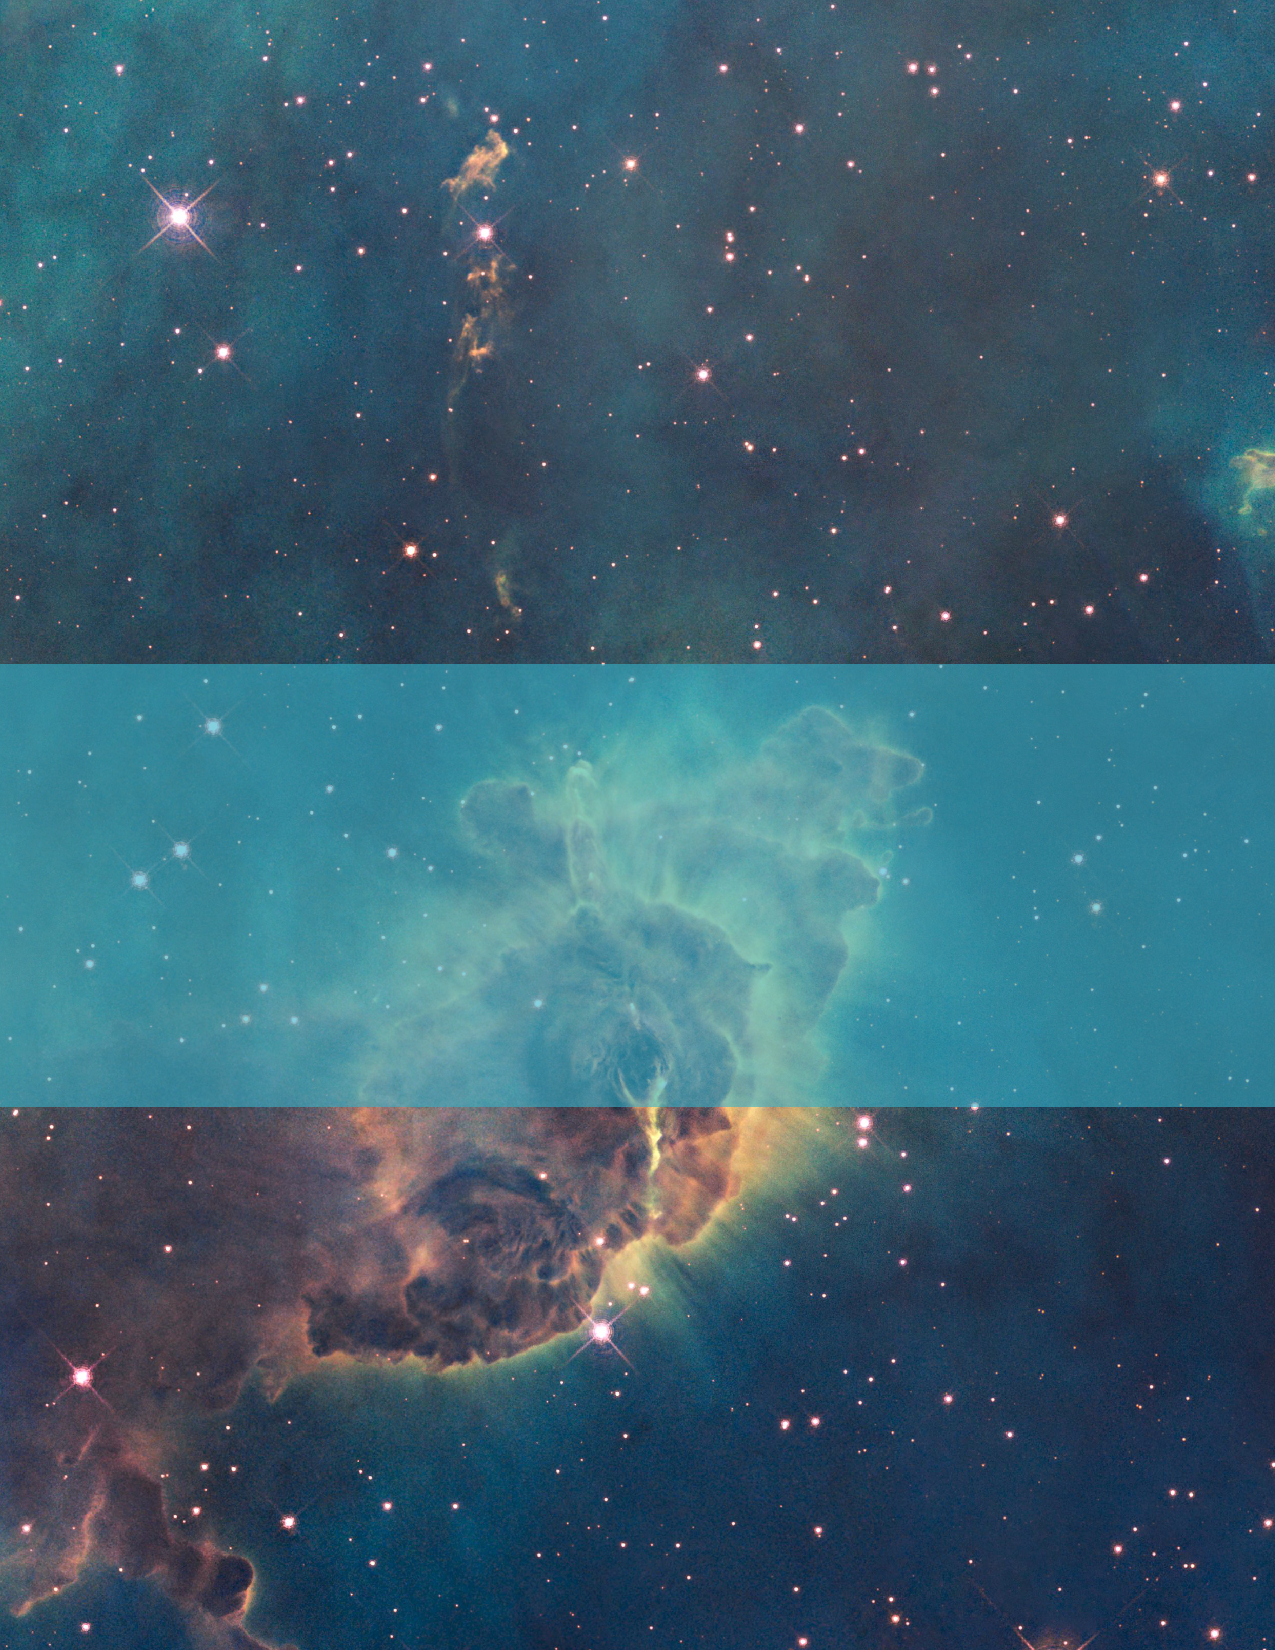
\includegraphics[scale=1.25]{esahubble}}} % Image background
\centering
\vspace*{5cm}
\par\normalfont\fontsize{35}{35}\sffamily\selectfont
\textbf{A Mathematical path to Engineering}\\
{\LARGE A Constructive Decalogue of formulas and recipes}\par % Book title
\vspace*{1cm}
{\Huge Rodrigo Ramele}\par % Author name
\endgroup

%----------------------------------------------------------------------------------------
%	COPYRIGHT PAGE
%----------------------------------------------------------------------------------------

\newpage
~\vfill
\thispagestyle{empty}

%\noindent Copyright \copyright\ 2014 Andrea Hidalgo\\ % Copyright notice

\noindent \textsc{Centro de Inteligencia Computacional, Instituto Tecnológico de Buenos Aires}\\

\noindent \textsc{github.com/faturita/path-to-engineering}\\ % URL

\noindent These notes have been gathered to 20 years of career.

\noindent \textit{First release, yet do not know} % Printing/edition date

%----------------------------------------------------------------------------------------
%	TABLE OF CONTENTS
%----------------------------------------------------------------------------------------

\chapterimage{head1.png} % Table of contents heading image

\pagestyle{empty} % No headers

\tableofcontents % Print the table of contents itself

%\cleardoublepage % Forces the first chapter to start on an odd page so it's on the right

\pagestyle{fancy} % Print headers again

%----------------------------------------------------------------------------------------
%	CHAPTER 1
%----------------------------------------------------------------------------------------

\chapterimage{head2.png} % Chapter heading image

\chapter{Introduction}

\section{Motivation}\index{Motivation}


Sometimes we get lost on the true origin of Engineering.
Which is the practical implementation of mathematics.  Since my entrance course to Engineering as undergraduate students, I started to gather mathematical notes.  This motivation came as a suggestion from Professor .
The number 3 sheets are very old by now, and they are really rotting, but I found that those notes are a one-to-one mapping of the structure in my brain where I think I understand those concepts.  If you are here to get a deep understanding of many concepts, this is not the place.  I happen to be a very good generalist, and I try to tackle broadly as general as I can, and I only deep digger in few areas.  I tried always to catch the underlying idea, the key concept.  Well, I failed.  In general, I couldn't do this.  Anyway, these notes helped me a lot, and I found that it also helped others, particularly my students and colleagues.

Additionally, if I manage to write everything, I can add references of papers and book, everything in one place, which will be very handy for me.

I abuse the word Engineering too much.  It is so vast, so big, so complex at the same time that there are huge areas that I am missing in this book.  This notes inevitably have my own approach to this area.  Like a hiker going up to the mountain, they only see their own side.   However there is something that I would like to point out.  And that is the spirit of engineering, their soul:  get the foundations, understand the problem, find a match in the foundations, get data, get more date, try to get a ground on what do you think, tinckle something, hack it, try to fix it. If nothing works use WD40 and duct tape.

Engineering is grounded in science, but I think it understands more humbly how the world operates, and the futility, in some way, of our actions.  That is way, it has a certain pragmatism, at the end, that is much more closer to nature than science itself.  Science is sometimes more pedantic, believing it can understand Nature, but you know of course, that Nature cannot be fooled. QUOTE !


\section{Objective}\index{Objective}

The purpose of this work is to establish in a step by step and constructive fashion a set of mathematical concepts from a pragmatic point of view, of mathematical ideas that are useful to engineering.

Everything that is written here is exactly what I understand. If anything is besides this notes, I just put it in the category of "Not-understanding".  

What I found is that I came to this notes, many times, adding more information and connections to other things, and I will always understand the same things from a different and completely new perspective.

After a while I found that I will be very disappointing of loosing those notes so I decided to write them down digitally. And have a backup with that.

How can you translate something that you created with your own pen ?  from your own handwriting ?  into something digital that is feel so cold to the naked eye.

Someone may found these notes useful.  I believe that will be for two reasons:  I wanted to create them in a constructive way: if I cannot find some rule to justify what I am doing then I am not doing anything, it doesn't exist.  The second reason is that I always found mathematics to be hard.  I love to understand it but it takes time to do it, to sit down.  At the same time, "undestanding" is not binary.  The best analogy I found is like a complex and evolutive graph or a tree-like structure, with many branches.  Let's say you understand something.  Then you have only "one path" to go from point A to point B of the concept.   But you can only walk across that path, and you, somehow, can follow the train of thinking from one place to the other.  However you cannot connect it to other things.  When you teach, somebody may point out the existence of point C closer to both.  But you were completely unaware of it until some student ask you something about it.  Then you discover that connection (and manage to give a response to the poor student, which it will be satisfactory or just mumble jamble).  Then you start to discover many more ramificiations and your level of understanding increases.  So understanding, is the level of ramification that you know of something, how much can you connect the concept to others.   

for Control engineerings for instance, everything can be a control problem.  The same can be applied to the "Rule of 3" or proportions or fractions.  Or algebra.  These very important tools allows you to tackle problems that is the reason they are so ubiquous.  In such way the Consciousness theory share some intuition with these concepts, measuring the level of integration and connectivity (Rhythms of the brain).



\subsection{References}\index{References}

Since I found so much good information about pretty much everything I wanted to know about, I will just create a remark and let you know where you can find more specific information about, just like below.

\begin{remark}
For more information about the cosmological principle, review Chapter 1: Why Learn Astronomy?, page 10, from \textbf{21st Century Astronomy}, \textit{Hester | Smith | Blumenthal | Kay | Voss}, Third Edition, 2010.
\end{remark}

%This statement requires citation \cite{book_key}; this one is more specific \cite[122]{article_key}.


%----------------------------------------------------------------------------------------
%	CHAPTER 2
%----------------------------------------------------------------------------------------
\chapterimage{band1.png}

\chapter{Set Theory: preliminaries}

%----------------------------------------------------------------------------------------
%	CHAPTER 3
%----------------------------------------------------------------------------------------

\chapterimage{boat.png}
\chapter{Precalculus}

The best book of Precalculus is Zill \cite{ZillBook}.  I will recommend this book to anyone to have a grasp on the mathematics that is in general required to enter Universities.

Zill has another book on complex analysis which is also great.  You will have to wait for complex numbers until we get signal processing, because I believe is their real place in Engineering. 


%----------------------------------------------------------------------------------------
%	CHAPTER 4
%----------------------------------------------------------------------------------------

\chapterimage{head1.png} % Chapter heading image

\chapter{Signal Processing}

\section{Qualitative Analysis}

\section{Complex Numbers}

\begin{equation}
z = (x, y)
\label{eq:c1}
\end{equation}


\begin{equation}
Re \; z = x
\label{eq:c1}
\end{equation}


\begin{equation}
Im \; z = y
\label{eq:c1}
\end{equation}

\section{Further work}
Well, finally we reached the point where I my time in Canada finished and I this research is still on its first stages. I have so many ideas of how to explore the clustering techniques in the DAME platform, MatLab, Python and everything else that can be tested \cite{Linde2012}

\chapter{Number Theory}

By far, the most interesting part of Number Theory is Hardy's quote:

This branch of mathematics will never be touch by the mundane pragmatism.

Or something like that.  Well, dear Hardy, you were right but you are now wrong.  This branch of mathematics has found in Cryptography one enormous directo applicaton of mathematics.  Such is this case, that if one very fundamental problem of mathematics like finding quickly and efficiently the primes factors of a really big number is theoretically tackled, it will immediate bring down half of ecomerce operations worldwide, will destroy companies, and will cost huge amount of money.  Anyway, this will never happen. 

\chapter{Pragmatic Control Theory}

That thing you are doing is called proportional control. \cite{book_key}.

\chapter{Introduction}
%\addcontentsline{toc}{chapter}{Introduction}  

%\textit{The cognitive computational process of agency does not reside exclusively on the internal physiological mechanism that sustain it, it requires a fluid active interaction with the environment in which it is located.  The limits of the mind are not determined by the material border, they extend across the environment, across the bubble which is feasible to be sensed, where the agent is physically located.  When this interaction is interrupted, it must be restored and enhanced when it is possible.}

%\quotation{ \textit{...the brain is not a passive decoder of information but a dynamic and distributed modeler of a reality comprised of a multitude of feedback, local, modulatory, and feedforward neural pathways conjuring a vast and elaborate organic spatiotemporal grid \cite{nicolelis2011beyond}} } \\

The brain is a machine with the sole purpose to respond appropriately to external and internal events, and to spread its own presence into the environment where it belongs~\footnote{The sensorimotor Hipothesis \cite{young1970,WolpawJonathanR2012} and The Extended Mind Thesis \cite{clark2008}}.  Hence, the brain needs to communicate and it possesses mainly two natural ways to do it: hormonal or neuromuscular.  When those natural channels are interrupted, they are not available or when it needs to increase or enhance the communication alternatives, a new artificial communication channel which is not based on natural pathways, is needed. It is based, instead, on a new technology feat that decodes the information from the CNS and transmits it directly to a computer or machine.

Brain Computer Interface, BCI, is a system that measures brainwaves and converts them into artificial output that replaces, restores, enhances, supplements and improves natural brain output and changes the ongoing interactions between the Central Nervous System and its external or internal environment \cite{WolpawJonathanR2012}. Brain Machine Interface (BMI) generally refers to invasive devices. Brain Neural Computer Interfaces (BNCI) may refer to devices that do not exclusively use information from the CNS, they also may use any kind of biological signal that can be harnessed with the purpose of volitionally transmit information. In essence, every kind of BCI system is after all a communication device.

%\marginpar{Above all, BCIs are communication devices.}

There are five motives behind BCI: the \textbf{first} is the aging of societies: estimated for 2025, 800 millions people will be over 65 years old, and $2/3$ of them on developing countries \cite{Lloyd-Sherlock2000}.  This may lead to an increased tendency to develop diseases that affect motor pathways and require some form of assistance from technology.  The \textbf{second} reason is the digital world that calls for more methods of interaction. This digital society~\cite{Dyson1998} demands more mechanisms to interpret the surrounding world and to translate human intentions through digital gadgets.  Additionally, the advancement of smart wearable devices that can be used over the skin is also pushing the frontiers to go deeper into the body to find there useful information.  The \textbf{third} motive is the impulse of neuroscience research and the advances that this discipline is having worldwide.  The \textbf{fourth} reason is the potentialities of BCI as a clinical tool which can help to diagnose diseases, as aid in the field of neurorehabilitation,  or to provide neurofeedback.  The \textbf{fifth}, final and most important motive, the reason behind Brain Computer Interfaces, is the still unfulfilled societal promise of social inclusion of people with disabilities.  It is known that the ability to walk and live independently is a key indicator of psychological and physical health, and we have to do all we can to provide the technological tools to achieve this goal~\cite{Rao2013,Clerc2016,WolpawJonathanR2012,Huggins2015}. 

In line with the aforementioned motives, there are several applications currently under development for BCI.  People affected by any kind of neurodegenerative diseases, particularly those affected by advanced stages of Amyotrophic Lateral Sclerosis (ALS) with locked-in syndrome may find in BCIs the only remaining alternative to communicate. Other applications targeted for the general population include alertness monitoring, telepresence, gaming, education, art, human augmentation~\cite{Yuste2017}, biometric identification, virtual reality avatar, assistive robotics and education.  Novel niches where this new communication channel can be useful are found routinely~\cite{Nam2018}. In spite of all this hype~\cite{GartnerHype2016}, there is still a long way ahead.  This area advanced rapidly but the complexity of brain signals in all their forms is still a big problem to tackle.  

%If you are a newcomer to this discipline a word of warning: there is still a long way ahead. 

%There are two types of BCIs.  Invasive and Noninvasive.  The first one involves 

%The traditional clinical approach consisted in analyzing the paper strip that was generated by the plot of the signal obtained from the device.  Expert technician and physicians analyzed visually the plots looking for specific patterns that may give a hint of the underlying cognitive process or pathology.   Atlases and guidelines were created in order to help in the recognition of these complex patterns.   Even Video-electroencephalography scalp recordings are routinely used as a diagnostic tools \cite{Giagante2003} .  The clinical EEG research has also focused on temporal waveforms, and a whole branch of electrophenomenology has arisen around EEG \textit{graphoelements} \cite{Schomer2010}.  

Electroencephalography (EEG) is the most widespread technique to capture electrical brain information in a non-invasive and portable way, and it is the most used device in BCI research and applications.  The clinical and historical tactic to analyze EEG signals were based on detecting visual patterns out of the EEG trace or polygraph~\cite{Hartman2005}: multichannel signals were extracted and continuously plotted over a piece of paper. Electroencephalographers or Electroencephalography technician have decoded and detected patterns along the signals by visually inspecting them~\cite{Schomer2010}.   Nowadays clinical EEG still entails a visually interpreted test~\cite{Hartman2005}.

In contrast, automatic processing, or quantitative EEG, was based first on analog electronic devices and later on computerized digital processing methods \cite{Jansen1991}.  They implemented mathematically and algorithmically complex procedures to decode the information with good results \cite{Yuste2017}.  The best materialization of the automatic processing of EEG signals rests precisely in the BCI discipline, where around $71.2\%$ is based on noninvasive EEG \cite{Guger2017}.  

%rich clinical literature

Hence, the traditional strategy of analyzing the electroencephalography by signal shapes on plots, was mainly neglected in BCI research, and the waveform of the EEG was replaced by procedures that were difficult to link to existing clinical EEG knowledge.  

%What if we could develop an automatic processing procedure which mimic how human beings interpret waveforms and analyze EEG in that same manner ?

On the other hand, the study of biological visual sensory system provided insights and models that are very useful to understand brain functions.  Additionally, they serve as inspiration to develop Computer Vision algorithms that intended to reproduce a similar level of accuracy as those obtained by biological beings, including humans.  The Histogram of Gradient Orientations is one successful method from Computer Vision useful to image recognition that aims to mimetically reproduce how the visual cortex discriminate shapes.

This thesis tries to unravel the following question:  is it possible to analyze and discriminate electroencephalographic signals by automatic processing the shape of the waveforms using the Histogram of Gradient Orientations ?

%To do that, I humbly ask the reader to join me in this brief journey: 

To do that, this work unfolds as follows: Chapter~\ref{chapter:one} gives details of what is a Brain Computer Interface and the particularities of the first window of the electric mind: the EEG. It also covers the state of the art in the methods that explore the waveform automatically.  Chapter \ref{chapter:two} provides an overview on the procedure to construct a plot representing the signal. Chapter \ref{chapter:three} is the core of this thesis and describes the Histogram of Gradient Orientations and how it can be used to process one-dimensional signals.
Next, results and experimental procedures are described to analyze EEG signals and implement BCI paradigms:  Alpha Waves are covered in Chapter \ref{chapter:four} and Motor Imagery in Chapter \ref{chapter:five}. The P300 Wave is studied in Chapter \ref{chapter:six}.  Future Work and Conclusions are addressed in Chapter~\ref{chapter:seven}.  

%Finally, appendixes provide extra additional information regarding the state-of-the-art of this discipline in Argentina, and also outlines particularities of the SIFT method and the theory behind the Histogram of Gradient Orientations of Signal Plots.

\section{Significance}

This thesis propose

\begin{itemize}
\item A procedure to construct analyzable 2D-images based on one-dimensional signals.
\item An enhancement over the Histogram of Gradient Orientation technique to allow non-squared patches and to adapt it to signal plots.
\item A mapping procedure to link EEG time-series characteristics to features of 2D-images.
\item A feature extraction method for EEG signals that can be used objectively to encode a representation of the waveform.
\item A classification algorithm that use the encoded representation with the purpose of comparing and identifying waveforms for BCI applications.
\end{itemize}

\section{Summary}

\begin{itemize}
\item What is this all about? A method to analyze EEG signals based on extracting local features from their 2D image plot representation.
\item What will be found in this thesis? A point of view that emphasizes the importance of providing mechanisms that help to understand signals based on how they look like on plots.
\item Does it work? It works when the waveform contains the discriminating information.  If a person is able to discriminate the signals, this method would also do that.
\item Can it be used?  Yes, it can.  The developed software is open-source and it can be used out-of-the-box.  It is particular useful when an intelligible automatic classification procedure is required.
\end{itemize}



\printbibliography

\end{document}


